%\documentstyle[epsf,twocolumn]{jarticle}       %LaTeX2e仕様
\documentclass[twocolumn]{jarticle}     %pLaTeX2e仕様(platex.exeの場合)
% \documentclass[onecolumn]{ujarticle}   %pLaTeX2e仕様(uplatex.exeの場合)
%%%%%%%%%%%%%%%%%%%%%%%%%%%%%%%%%%%%%%%%%%%%%%%%%%%%%%%%%%%%%%
%%
%%  基本バージョン
%%
%%%%%%%%%%%%%%%%%%%%%%%%%%%%%%%%%%%%%%%%%%%%%%%%%%%%%%%%%%%%%%%%
\setlength{\topmargin}{-45pt}
%\setlength{\oddsidemargin}{0cm}
\setlength{\oddsidemargin}{-7.5mm}
%\setlength{\evensidemargin}{0cm}
\setlength{\textheight}{24.1cm}
%setlength{\textheight}{25cm}
\setlength{\textwidth}{17.4cm}
%\setlength{\textwidth}{172mm}
\setlength{\columnsep}{11mm}

%\kanjiskip=.07zw plus.5pt minus.5pt


% 【節が変わるごとに (1.1)(1.2) … (2.1)(2.2) と数式番号をつけるとき】
%\makeatletter
%\renewcommand{\theequation}{%
%\thesection.\arabic{equation}} %\@addtoreset{equation}{section}
%\makeatother

%\renewcommand{\arraystretch}{0.95} 行間の設定
%%%%%%%%%%%%%%%%%%%%%%%%%%%%%%%%%%%%%%%%%%%%%%%%%%%%%%%%
%\usepackage{graphicx}   %pLaTeX2e仕様(\documentstyle ->\documentclass)
\usepackage[dvipdfmx]{graphicx}
\usepackage{subcaption}
\usepackage{multirow}
\usepackage{amsmath}
\usepackage{url}
\usepackage{ulem}
\usepackage{algorithm}
\usepackage{algorithmic}
\usepackage{listings} %,jlisting} %日本語のコメントアウトをする場合jlistingが必要
%ここからソースコードの表示に関する設定
\lstset{
  basicstyle={\ttfamily},
  identifierstyle={\small},
  commentstyle={\smallitshape},
  keywordstyle={\small\bfseries},
  ndkeywordstyle={\small},
  stringstyle={\small\ttfamily},
  frame={tb},
  breaklines=true,
  columns=[l]{fullflexible},
  numbers=left,
  xrightmargin=0zw,
  xleftmargin=3zw,
  numberstyle={\scriptsize},
  stepnumber=1,
  numbersep=1zw,
  lineskip=-0.5ex
}
%%%%%%%%%%%%%%%%%%%%%%%%%%%%%%%%%%%%%%%%%%%%%%%%%%%%%%%%
\begin{document}

	%bibtex用の設定
	%\bibliographystyle{ujarticle}

	\twocolumn[
		\noindent
		\hspace{1em}
		2020 年 11 月 27 日
		ゼミ資料
		\hfill
		B4 杉山 竜弥
		\vspace{2mm}

		\hrule
		\begin{center}
			{\Large \bf 進捗報告}
		\end{center}
		\hrule
		\vspace{9mm}
	]

\section{今週やったこと}
\begin{itemize}
  \item GAの実装と実験
\end{itemize}

\section{実験}

\subsection{問題}
DARTSの初期値依存性やグラフの収束不安定のためGAを使用する.
個体をアーキテクチャ$\alpha$とし, $w$を共有することで,
学習速度を維持しつつ, 学習の安定を図る.

評価の問題
\begin{itemize}
  \item 通常:与えられたパラメータ(個体)でモデルを学習し性能を評価する
  \item 今回:$w$を共有するので呼ぶごとに評価が変化する
\end{itemize}

\paragraph{GAの流れ}
$\alpha$, $w$の学習はアーキテクチャ探索として分離して,
評価では$\alpha$, $w$に変化を与えずテストデータのロスを用いる.
% (memo 評価前の適応度で選択しているのはまずい)
\begin{enumerate}
  \item 初期化
  \item (アーキテクチャ探索)
  \item 選択
  \item 交叉・突然変異
  \item 評価・世代交代
\end{enumerate}

\paragraph{$\alpha$の個体表現}
$\alpha$は行列であるため, 交叉をどうするかが難しい.
初期段階の方法として, 行列を2次元配列にして2点交叉をした.
何が適しているかを調査する必要がある.

\subsection{実験設定}

\begin{table}[tb]
  \begin{center}
    \caption{モデルの設定}
    \begin{tabular}{|c|c|} \hline
      base model & VGG19 \\ \hline
      Optim($w$) & SGD(lr=0.001, momentum=0.9) \\ \hline
      Optim($\alpha$) & Adam(lr=0.003, $\beta$=(0.5, 0.999)) \\ \hline
      Loss & Cross Entropy Loss \\ \hline
      dataset & cifar10 \\ \hline
      pretrain & true \\ \hline
      batch size & 64 \\ \hline
      train size & 2500 \\ \hline
      valid size & 2500 \\ \hline
    \end{tabular}
    \label{tab:setting}
  \end{center}
\end{table}

\begin{table}[tb]
  \begin{center}
    \caption{GAの設定}
    \begin{tabular}{|c|c|} \hline
      個体数 & 10 \\ \hline
      世代数 & 10 \\ \hline \hline
      選択 & トーナメント \\ \hline
      サイズ & 3 \\ \hline \hline
      交叉 & 2点交叉 \\ \hline
      交叉率 & 0.5 \\ \hline \hline
      変異 & ガウス分布 \\ \hline
      変異率 & 0.2 \\
      (遺伝子座ごと) & 0.1 \\ \hline
    \end{tabular}
    \label{tab:setting_ga}
  \end{center}
\end{table}

表 \ref{tab:setting}, \ref{tab:setting_ga} にモデルとGAの設定を示した.
前回までの設定ではショートカットを持たない状態で学習を始めるが,
GAの場合多様性がなくなるため各層に1本ずつ持たせる設定で学習した.

\subsection{結果}

図 \ref{fig:acc}, \ref{fig:loss} にGAの結果の精度とロスを示した.
ただしこの結果は$\alpha$から作成したモデルの性能ではないため,
本来の値とは異なる.
図では精度は世代ごとに向上するが, 2世代から損失は悪化した.
モデルが出力する確信度が平均的な$\alpha$に最適化された結果,
逆にすべての$\alpha$との差が損失に大きな誤差を与えたと思われる.

今回の設定の場合, 1世代にかかる時間は3分であった.
データをすべて使う場合, 1個体あたり3分となり, 20個体の場合1世代に1時間かかる.

\begin{figure*}[tb]
 \begin{minipage}{0.5\hsize}
 	\begin{center}
 		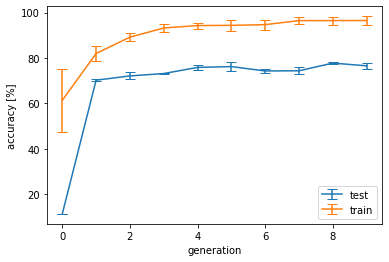
\includegraphics[clip,width=75mm]{acc.png}
 		\caption{世代ごとの精度 (平均と標準偏差)}
 		\label{fig:acc}
 	\end{center}
 \end{minipage}
 \begin{minipage}{0.5\hsize}
 	\begin{center}
 		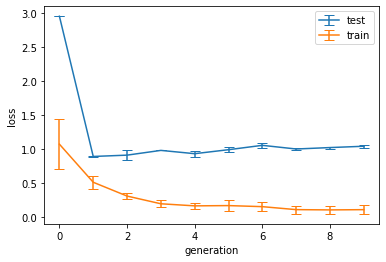
\includegraphics[clip,width=75mm]{loss.png}
 		\caption{世代ごとのロス (平均と標準偏差)}
 		\label{fig:loss}
 	\end{center}
 \end{minipage}
\end{figure*}

%
% \section{GAの準備}
% deapでサンプルのGAを動作を確認.
%
% 問題
% \begin{itemize}
%   \item 個体表現($\alpha$は行列)
%   \item 交叉・突然変異の方法
%   \item メモリに乗るか?
%   \item 実行時間
% \end{itemize}
% とりあえず今のDARTSのコードに実装してみる.
%
% \begin{figure*}[tb]
%  \begin{minipage}{0.333\hsize}
%  	\begin{center}
%  		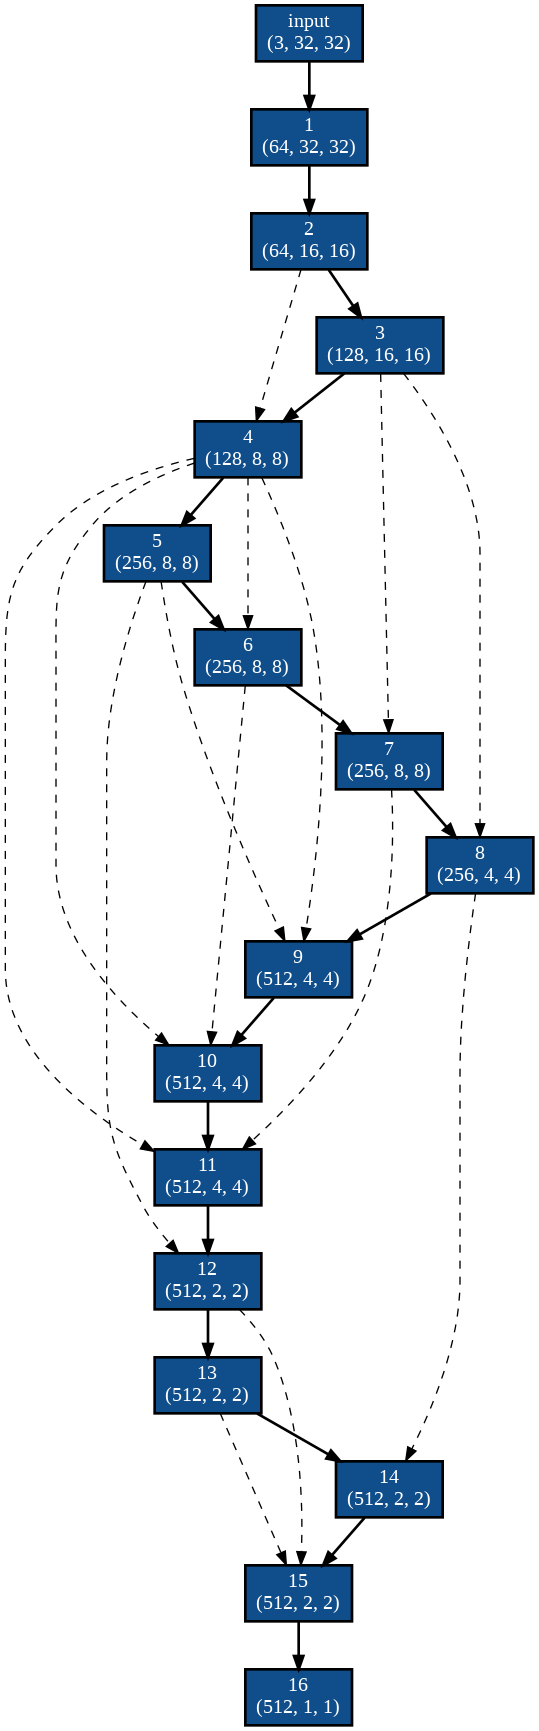
\includegraphics[clip,scale=0.25]{graph_50_search.png}
%  		\caption{手法Aのグラフ(50 epoch)}
%  		\label{fig:graph_s}
%  	\end{center}
%  \end{minipage}
%  \begin{minipage}{0.333\hsize}
%  	\begin{center}
%  		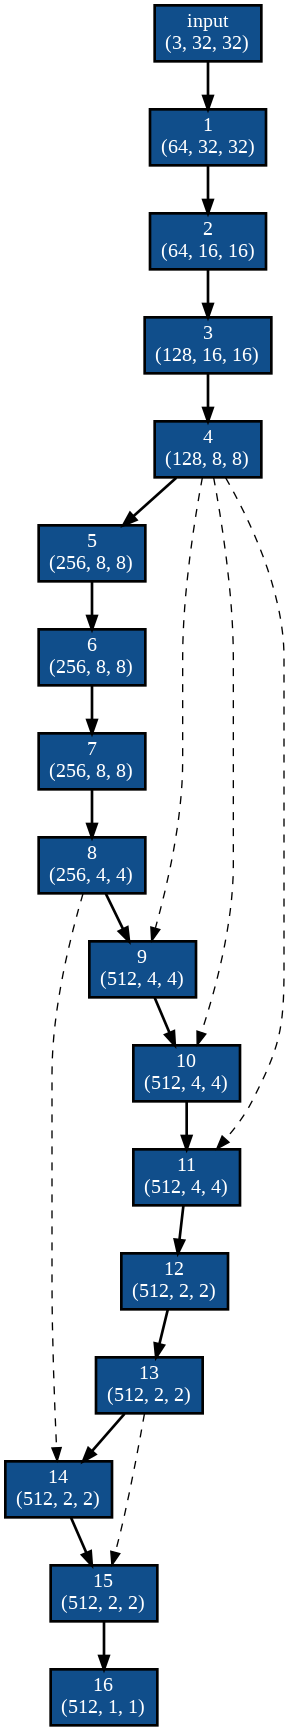
\includegraphics[clip,scale=0.25]{graph_50_search_edge.png}
%  		\caption{手法Bのグラフ(50 epoch)}
%  		\label{fig:graph_e}
%  	\end{center}
%  \end{minipage}
%  \begin{minipage}{0.333\hsize}
%  	\begin{center}
%  		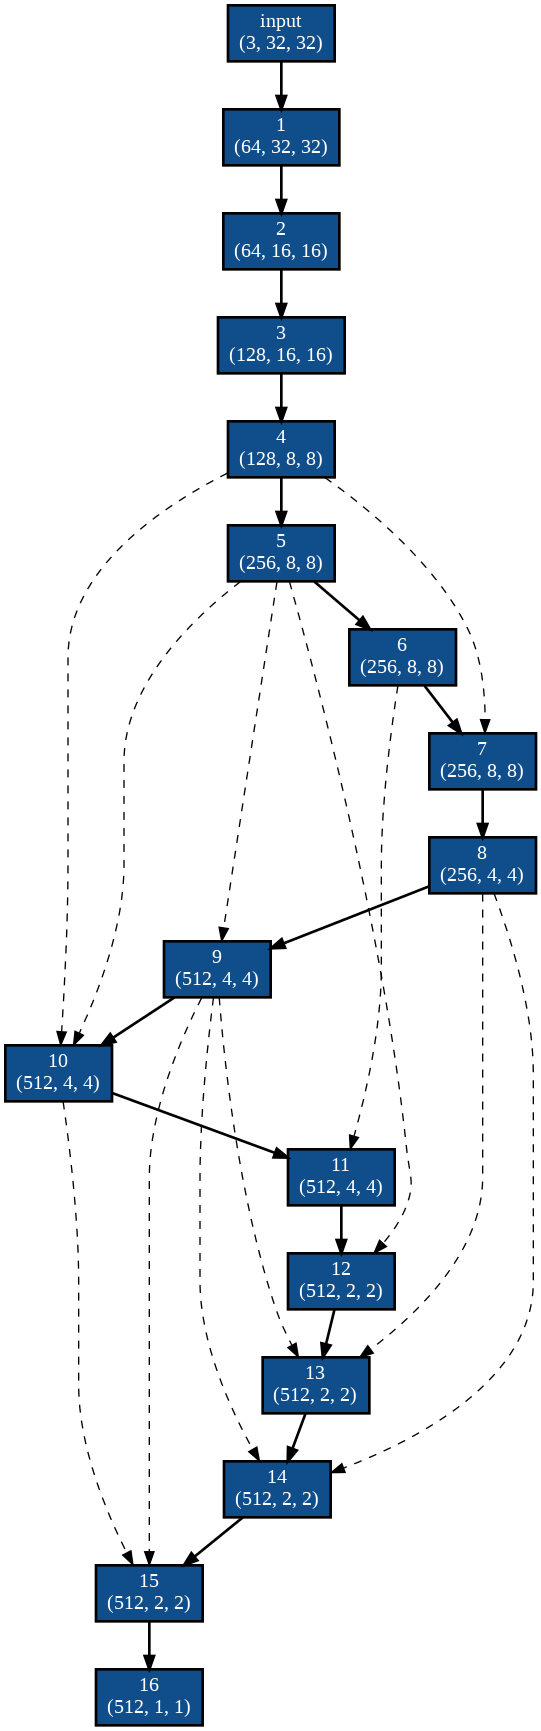
\includegraphics[clip,scale=0.25]{graph_50_pretrain_search.png}
%  		\caption{手法Aのグラフ(50 epoch, pretrained)}
%  		\label{fig:graph_p}
%  	\end{center}
%  \end{minipage}
% \end{figure*}
%
% \begin{figure*}[tb]
%  \begin{minipage}{0.5\hsize}
%  	\begin{center}
%  		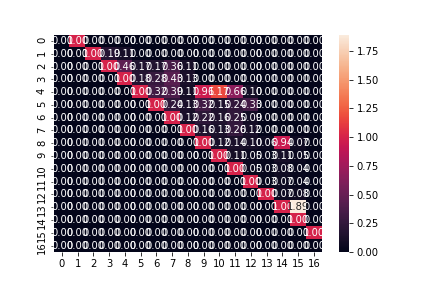
\includegraphics[clip,width=75mm]{alpha_50_search.png}
%  		\caption{事前学習なしの$\alpha$(従来)}
%  		\label{fig:alpha}
%  	\end{center}
%  \end{minipage}
%  \begin{minipage}{0.5\hsize}
%  	\begin{center}
%  		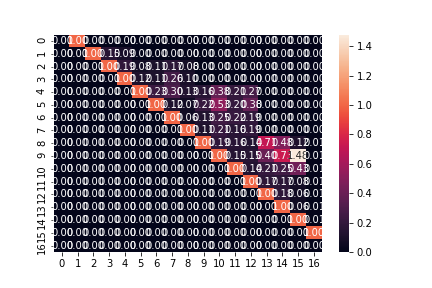
\includegraphics[clip,width=75mm]{alpha_50_pretrain_search.png}
%  		\caption{事前学習ありの$\alpha$(今回)}
%  		\label{fig:alpha_p}
%  	\end{center}
%  \end{minipage}
% \end{figure*}

\section{今後の予定}
% なんとなくなんかの勉強をするとかではなく具体的に

まずGAはメモリの問題もなく動いた.
しかし交叉や突然変異などは適した手法が分からないため,
GAを調査して設定を見直したい.
うまくいけば来週サーバーで長時間動かす.

\begin{itemize}
  % \item DARTのunrolling実験
\end{itemize}

\section{ソースコード}
% 埋め込みでもGitでもいいので参照できるように
githubのnotebookリポジトリ参照.

% 参考文献リスト
\bibliographystyle{unsrt}
\bibliography{ref}
\end{document}
